\chapter{Change Point Analysis}
\label{chap:change_point}

A few points:

\begin{itemize}
\item we are dealing with offline change point detection.
\item RUPTURE package can be used for change point analysis in python. It is very well documented, and the plots are good looking.
\item There are approximate and optimal ways for finding changing points. Since we don't have many points in our time series (roughly 50, for computational cost reasons), we decide to use the optimal algorithms.
\item I can write more about the difference and how it works.
\item I wish HATDEP improves the capacity of RUPTURE to catch the right time for the transition. However, it isn't that straightforward. When the kernels are all equal, symmetric and wide, there is a transition phase between the two behaviours. The best changing point is exactly in the middle and so the changing point is well captured. On the other hand, HATDEP improves in the MSE sense and might shift where the middle of the transition phase lies, yielding worst changing point detection.
\end{itemize}

références :

\cite{change_point_detection_these} and \cite{rupture_docu}, both very well documented and precise.

Pruned Exact Linear Time (PELT) search method: The PELT method is an exact method, and generally produces quick and consistent results. It detects change points through the minimization of costs. The algorithm has a computational cost of $O(n)$, where n is the number of data points. For more info on the PELT method, check out \cite{PELT_docu}

Dynamic programming search method: This is an exact method, which has a considerable computational cost of $O(Qn^2 )$, where $Q$ is the max number of change points and n is the number of data points. For more info on the dynamic programming search method, check out \cite{rupture_docu}.

Binary segmentation search method: This method is arguably the most established in literature. Binary segmentation is an approximate method with an efficient computational cost of $O (n log n)$, where n is the number of data points. The algorithm works by iteratively applying a single change point method to the entire sequence to determine if a split exists. If a split is detected, then the sequence splits into two sub-sequences. The same process is then applied to both sub-sequences, and so on. For more info on binary segmentation, check out \cite{binary_segmentation_change_point}.

Window-based search method: This is a relatively simple approximate search method. The window-based search method “computes the discrepancy between two adjacent windows that move along with signal. When the two windows are highly dissimilar, a high discrepancy between the two values occurs, which is indicative of a change point. Upon generating a discrepancy curve, the algorithm locates optimal change point indices in the sequence. For more info on the window-based search method, check out \cite{rupture_docu}



\begin{figure}
\centering
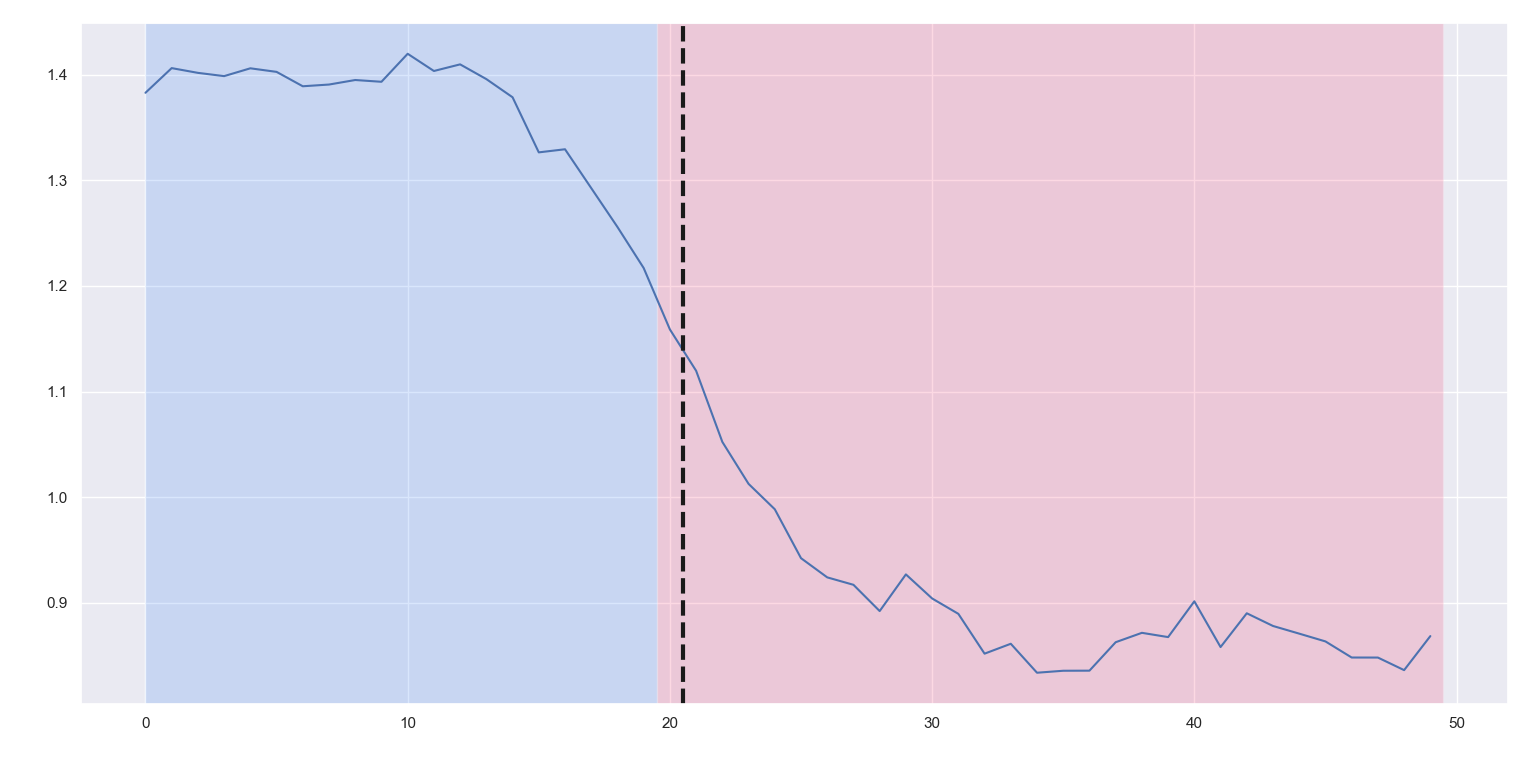
\includegraphics[width = 0.90 \textwidth]{../imag/chap4/Figure_2.png}
\caption{Changing point analysis. Simple jump data, the true phases are delimited by the colours, the dotted line shows where the transition is detected by RUPTURE. ALPHA.}
\label{fig:changing_point_2}
\end{figure}



\begin{figure}
\centering
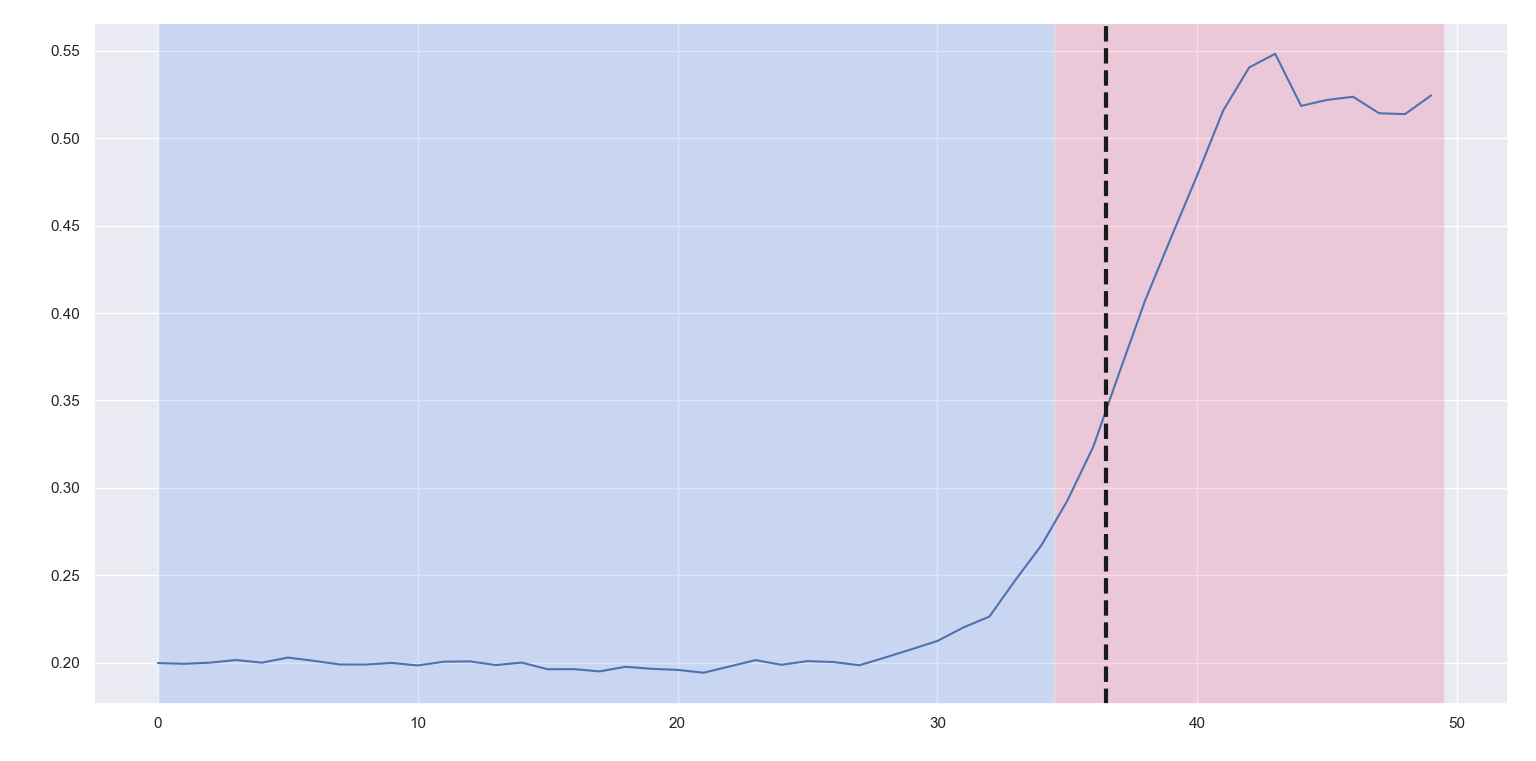
\includegraphics[width = 0.90 \textwidth]{../imag/chap4/Figure_4.png}
\caption{Changing point analysis. Simple jump data, the true phases are delimited by the colours, the dotted line shows where the transition is detected by RUPTURE. NU.}
\label{fig:changing_point_4}
\end{figure}




\begin{figure}
\centering
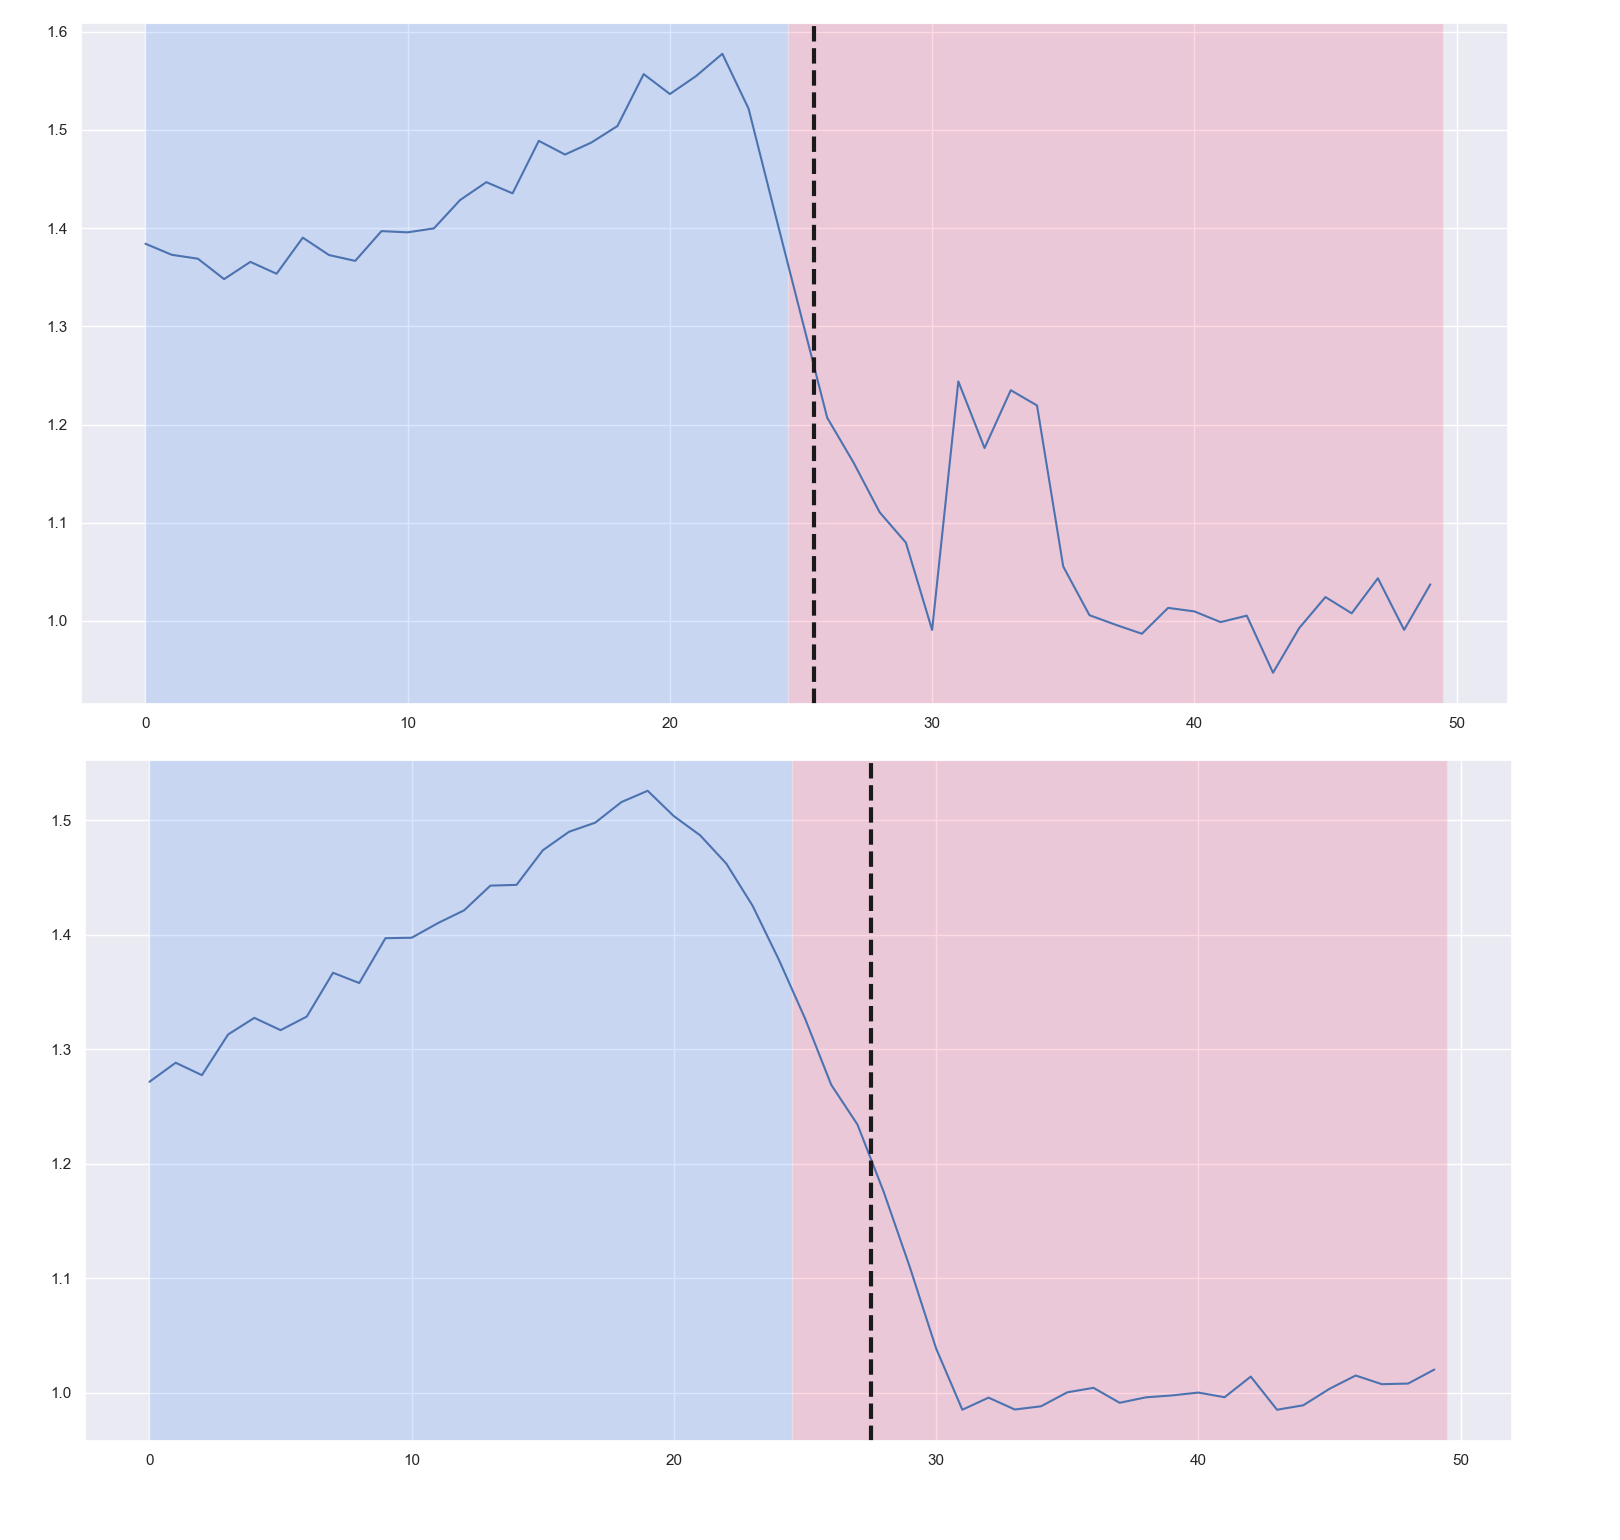
\includegraphics[width = 0.90 \textwidth]{../imag/chap4/Figure_22.png}
\caption{Changing point analysis. Simple jump and linear trend data, the true phases are delimited by the colours, the dotted line shows where the transition is detected by RUPTURE. We display the comparison between, at the top estimation after HATDEP, below before HATDEP. ALPHA.}
\label{fig:changing_point_22}
\end{figure}



\begin{figure}
\centering
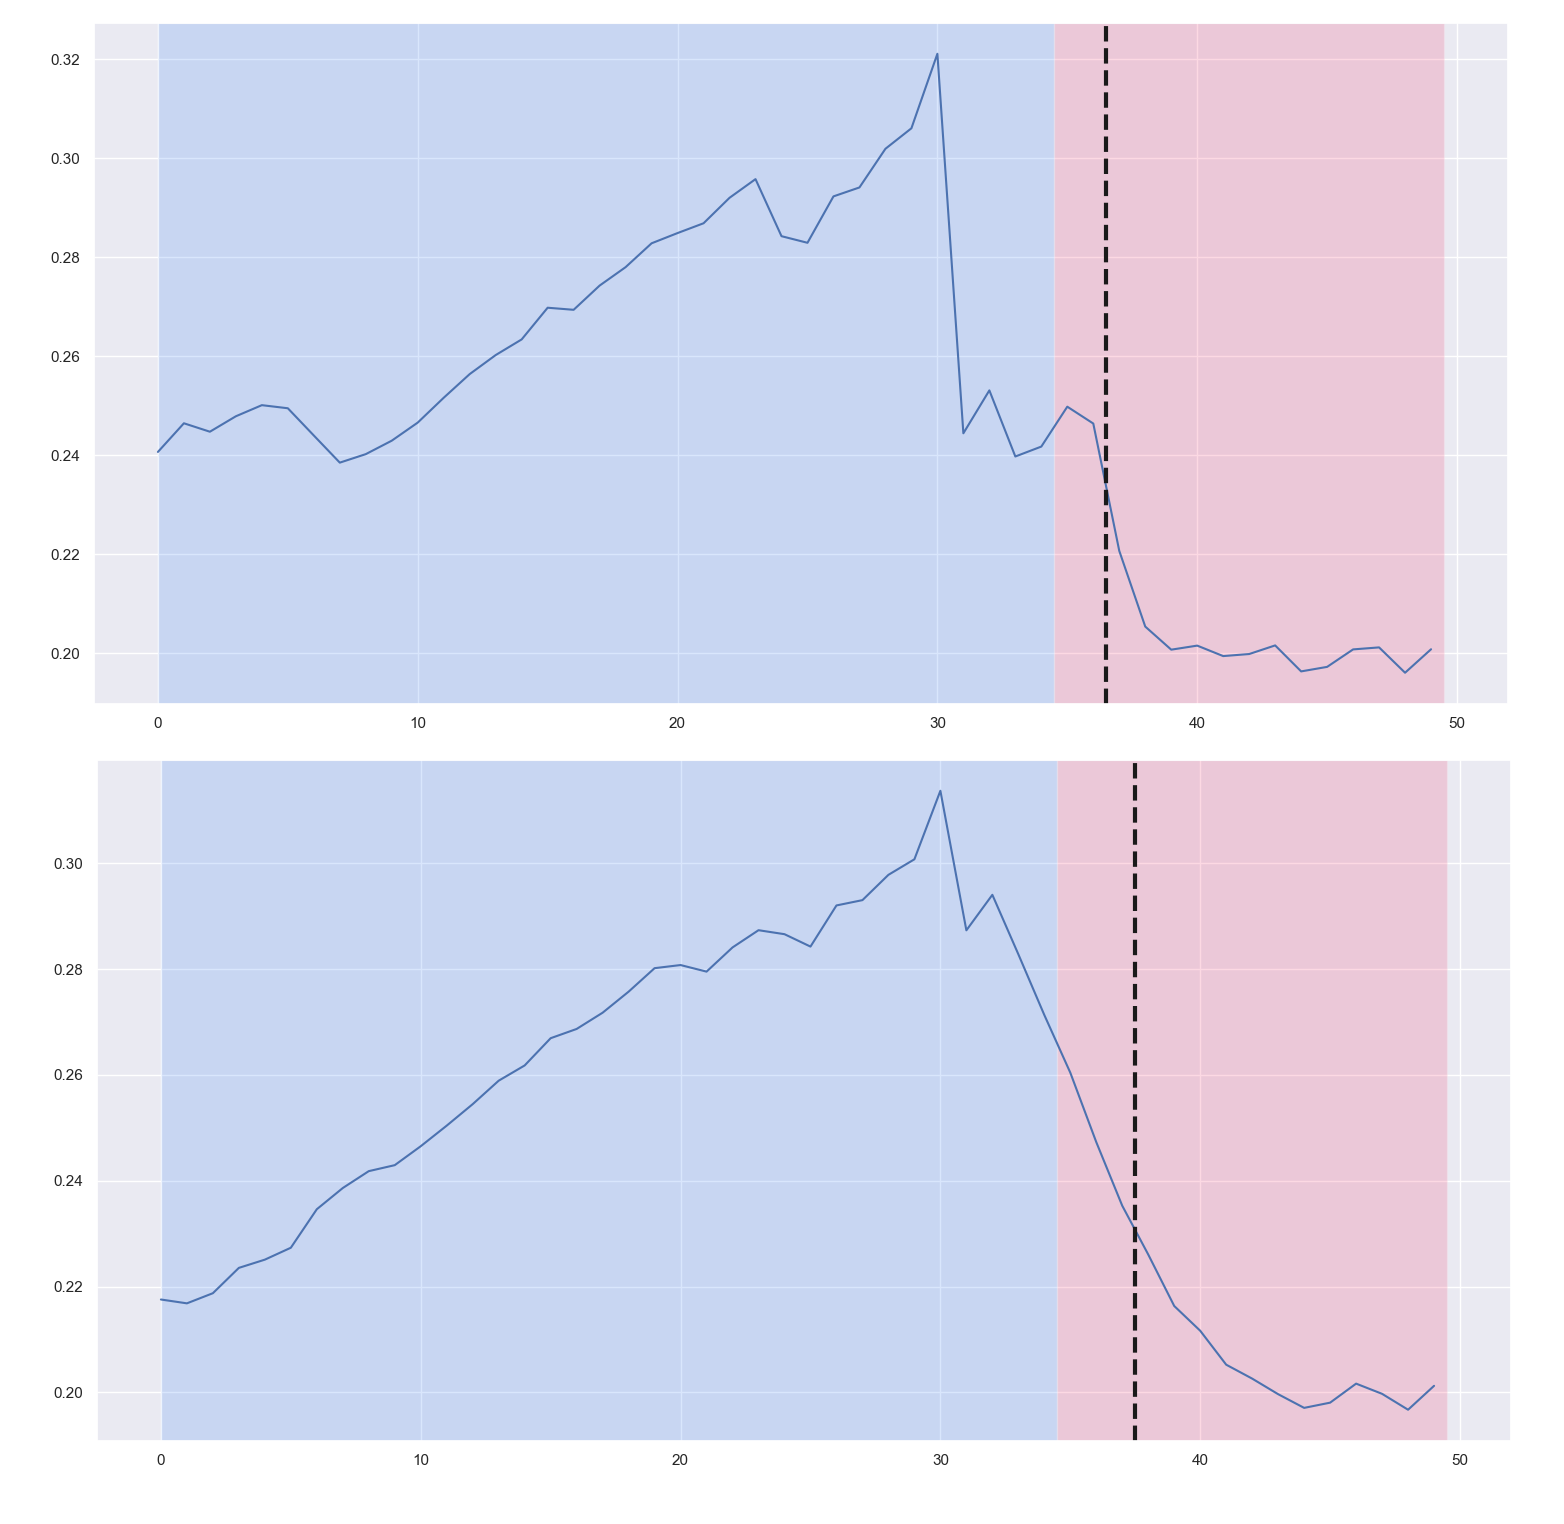
\includegraphics[width = 0.90 \textwidth]{../imag/chap4/Figure_42.png}
\caption{Changing point analysis. Simple jump and linear trend data, the true change point is written down by the dotted line, the two colours gives what RUPTURE detected. We display the comparison between, at the top estimation after HATDEP, below before HATDEP. NU.}
\label{fig:changing_point_42}
\end{figure}


\begin{figure}
\centering
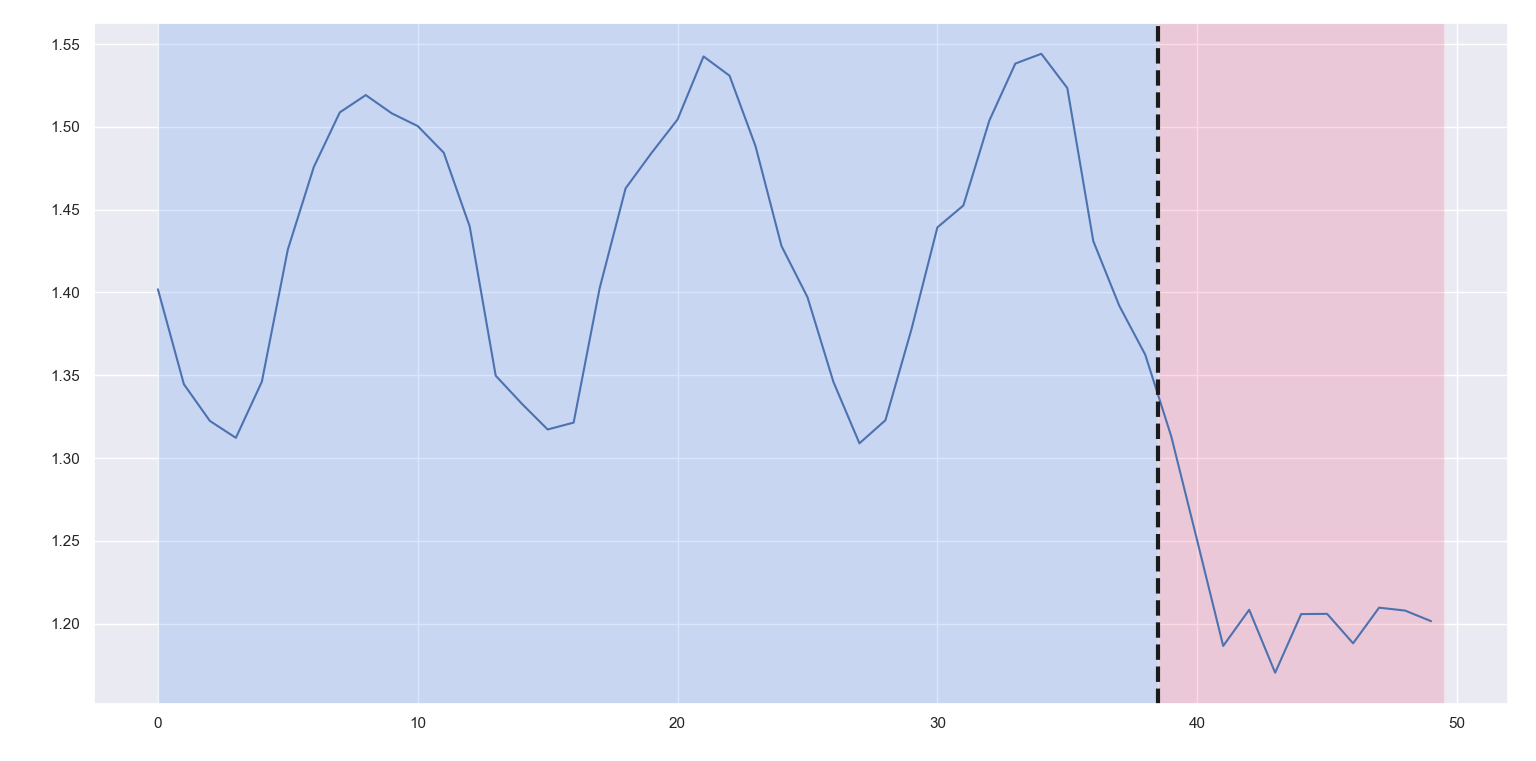
\includegraphics[width = 0.90 \textwidth]{../imag/chap4/Figure_222.png}
\caption{Changing point analysis. Sinusoidal data, the true change point is written down by the dotted line, the two colours gives what RUPTURE detected. ALPHA.}
\label{fig:changing_point_222}
\end{figure}

\begin{figure}
\centering
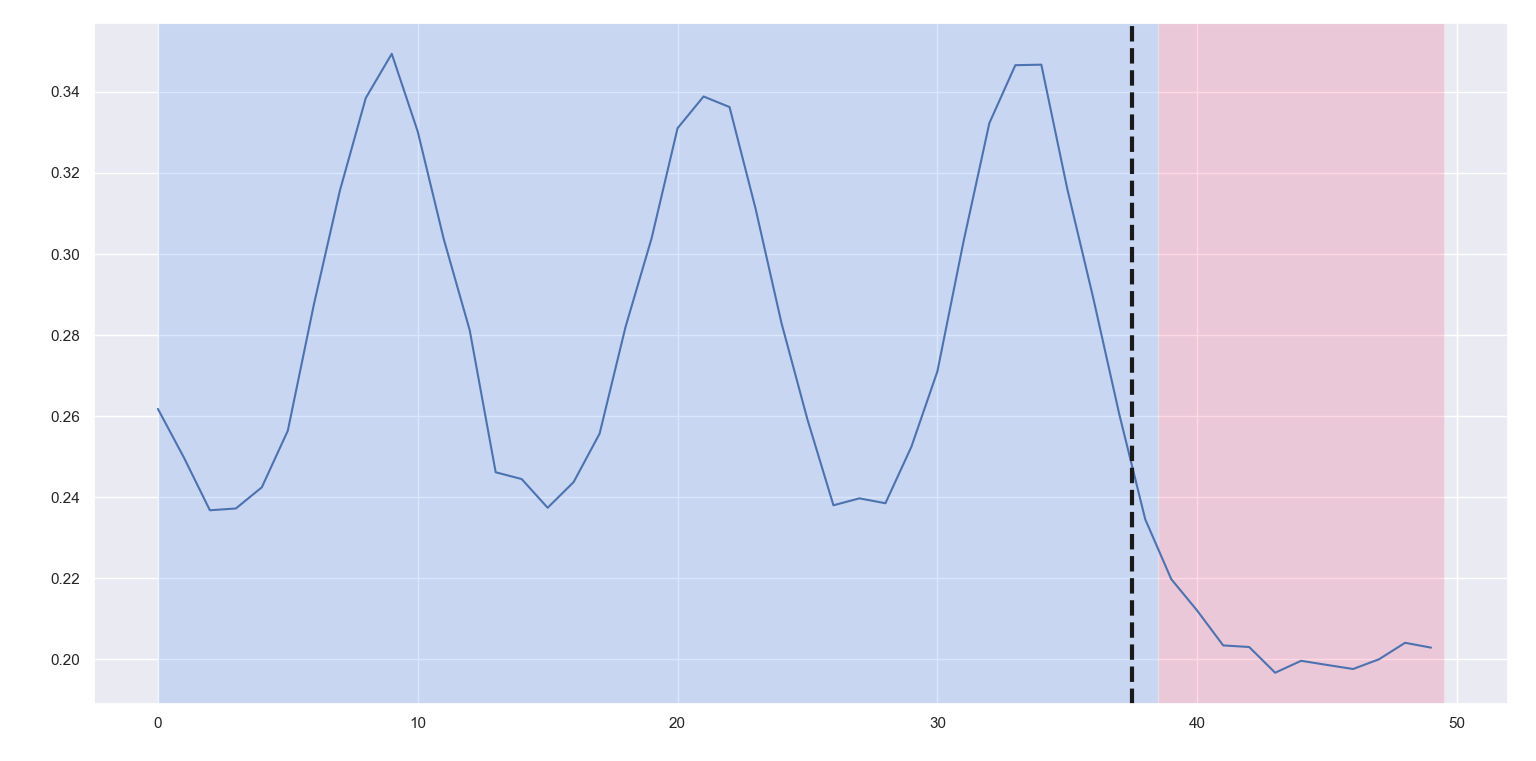
\includegraphics[width = 0.90 \textwidth]{../imag/chap4/Figure_422.png}
\caption{Changing point analysis. Sinusoidal data, the true change point is written down by the dotted line, the two colours gives what RUPTURE detected. NU.}
\label{fig:changing_point_422}
\end{figure}
